\documentclass[a4paper,10pt]{report}
\newcommand{\pmatrice}[1]{\begin{pmatrix}#1\end{pmatrix}}
\usepackage{cours}
\usepackage{pifont}

\begin{document}
\everymath{\displaystyle}
\begin{center}
\textit{{ {\huge TD 11 : Espaces probabilisés}}}
\end{center}

\bigskip


\begin{center}
\textit{{ {\large Dénombrement et dénombrabilité}}}
\end{center}

\medskip

\begin{Exercice}{} Calculer les sommes suivantes ($n \in \mathbb{N}$) : 
$$\dis\sum_{k=0}^n k \binom{n}{k}, \; \dis\sum_{k=0}^n\dis\frac{1}{k+1} \binom{n}{k} \; \hbox{ et } \; \sum_{k=0}^n \binom{2n+1}{k}$$
\end{Exercice}

\begin{Exercice}{} Soit $(p, n) \in \mathbb{N}^2$ tel que $p \leq n$. Déterminer la valeur de $\dis\sum_{k=p}^n{k\choose p} \cdot$

%={n+1\choose p+1}\cdot$
\end{Exercice}


\begin{Exercice}{}Soient $3$ urnes $U_1,U_2$ et $U_3$ et $n$ boules numérotées ($n \in \mathbb{N}^*$) de 1 à $n$.
\begin{enumerate}
\item Quel est le nombre total de répartitions de ces boules dans les trois urnes ?
\item Quel est le nombre total de répartitions qui laissent au moins $U_1$ vide ? au moins une urne vide ?
\item En déduire le nombre de répartitions qui ne laissent aucune urne vide.
\end{enumerate}
\end{Exercice}



\begin{Exercice}{} Un tiroir contient 5 paires de chaussures noires, 3 paires de chaussures vertes et 2 paires de chaussures rouges. Toutes les paires d'une même couleur ont des formes différentes. On prend deux chaussures au hasard simultanément dans le tiroir.
\begin{enumerate}
\item Combien y a-t-il de tirages possibles ?
\item 
Combien de tirages donnent :
\begin{enumerate}
\item deux chaussures de même couleur ?
\item un pied gauche et un pied droit ?
\item au moins un pied gauche ?
\item deux chaussures de la même couleur avec un pied gauche et un pied droit ?
\item une vraie paire de chaussures (deux chaussures de même couleur et même forme avec un pied gauche et un pied droit) ?
\end{enumerate}
\end{enumerate}
\end{Exercice}


\begin{Exercice}{\ding{80}}  Soit $f : \mathbb{N}^2 \rightarrow \mathbb{N}$ définie par :
$$ f((p,q)) = \frac{(p+q)(p+q+1)}{2} + q$$
\begin{enumerate}
\item Calculer $f((0,0))$, $f((1,0))$, $f((0,1))$, $f((2,0))$ et $f((1,1))$.
\item Représenter sur un schéma la manière dont $f$ liste les éléments de $\mathbb{N}^2$.
\item Nous souhaitons montrer que $\mathbb{N}^2$ est dénombrable. 
\begin{enumerate}
\item Soit $n \geq 0$. Justifier l'existence de :
$$ m_0 = \max \left\lbrace m \geq 0, \, \frac{m(m+1)}{2} \leq n \right\rbrace$$
Encadrer alors $n-\dfrac{m_0(m_0+1)}{2}$ et en déduire que $f$ est une surjection de $\mathbb{N}^2$ sur $\mathbb{N}$.
\item Montrer que $f$ est injective.
\item Conclure.
\end{enumerate}
\end{enumerate}
\end{Exercice}




\medskip

\begin{center}
\textit{{ {\large Équiprobabilité}}}
\end{center}

\medskip



\begin{Exercice}{} Un jeu de cartes comporte $32$ cartes. On tire simultanément $8$ cartes dans ce jeu de $32$ cartes. 

\begin{enumerate}
\item Quelle est la probabilité d'obtenir au moins un pique ?
\item Quelle est la probabilité d'obtenir exactement un pique ?
\item Quelle est la probabilité d'obtenir 2 carrés (un carré est constitué de 4 cartes de la même hauteur, par exemple 4 rois)?
\item Quelle est la probabilité d'obtenir un roi et un pique exactement ?
\end{enumerate}
\end{Exercice} 



\begin{Exercice}{Le problème des anniversaires}
On considère un groupe de $n$ personnes ($n \in \mathbb{N}^*$ avec $n \leq 365$).\\
Quelle est la probabilité qu'au moins deux personnes aient leur anniversaire le même jour ?
\end{Exercice}


\begin{Exercice}{} Une urne contient 5 boules blanches et 10 boules noires.

\begin{enumerate}
\item On tire au hasard successivement et avec remise 2 boules de l'urne.
\begin{enumerate}
\item Quelle est la probabilité d'obtenir une boule blanche et une boule noire dans cet ordre ?
\item Quelle est la probabilité d'obtenir une boule blanche et une boule noire dans un ordre quelconque ?
\end{enumerate}
\item Mêmes questions dans le cas de tirages sans remise.
\item On tire simultanément 5 boules de l'urne. Quelle est la probabilité d'obtenir 2 boules blanches et 3 boules noires ?
\end{enumerate}
\end{Exercice}





\medskip

\begin{center}
\textit{{ {\large Tribu et probabilité}}}
\end{center}

\medskip


\begin{Exercice}{\ding{80}}  Soit $\Omega$ un univers muni d'une tribu ${\cal A}$. On se donne un sous-ensemble $\Omega'$ de $\Omega$ et on pose :
 $${\cal A}'=\{A\cap \Omega',\ A\in{\cal A}\}$$
Montrer que ${\cal A}'$ est une tribu sur $\Omega'.$
\end{Exercice}


\begin{Exercice}{}  Soient $E,F$ deux évènements d'un même espace probabilisé.
\begin{enumerate}
\item Montrer que $P(E \cup F) \leq P(E) + P(F)$.
\item Soit $G$ un évènement. Montrer que $P(E \cup F \cup G) \leq P(E) + P(F) + P(G)$.
\item Écrire cette inégalité pour $\overline{E}$, $\overline{F}$ et $\overline{G}$ et en déduire que si $E,F$ et $G$ sont équiprobables de probabilité $p$ et si $P(E \cap F \cap G)=0$ alors $p \leq \dis \frac{2}{3} \cdot$
\end{enumerate}
\end{Exercice}




\begin{Exercice}{} Soient $n \geq 1$ et $(A_1, \ldots, A_n)$ une famille de $n$ évènements d'un espace probabilisé $(\Omega, \mathcal{A}, \P)$. Montrer que :
$$ \P(A_1 \cup \cdots \cup A_n) \leq \P(A_1) + \cdots + \P(A_n) \leq P(A_1 \cap \cdots \cap A_n) + n-1$$
\end{Exercice}



\begin{Exercice}{} Soit $(a_n)_{n \geq 0}$ une suite strictement décroissante de réels strictement positifs de limite nulle.  Déterminer $\lambda \in \R$ tel qu'il existe une probabilité $\P$ sur $\bigl(\N,\mathcal{P}(\N)\bigr)$ vérifiant :
    \[
    \forall n \geq 0, \qquad \P\bigl( \lbrace n, n+1, \ldots \rbrace) = \lambda a_n
    \]
\end{Exercice} 




\medskip

\begin{center}
\textit{{ {\large Probabilités conditionnelles}}}
\end{center}

\medskip

\begin{Exercice}{} On peut distinguer des élèves en trois catégories : ceux qui aiment la chimie, ceux qui n'aiment pas et ceux qui s'en fichent (royalement). Les étudiants des classes PC et PSI du lycée Robespierre sont assez différents : les étudiants en PC aiment la chimie avec une probabilité de $0.6$ et n'aiment pas avec une probabilité de $0.2$ alors que les étudiants en PSI aiment la chimie avec une probabilité de $0.4$ et s'en fichent avec une probabilité de $0.4$. On rencontre un étudiant au hasard et on suppose qu'il a deux fois plus de chance d'être en PSI plutôt qu'en PC.

\begin{enumerate}
\item Quelle est la probabilité qu'il aime la chimie?
\item Si il aime la chimie, quelle est la probabilité qu'il soit en PC?
\end{enumerate}
\end{Exercice}



\begin{Exercice}{} On considère deux urnes $U$ et $V$. L'urne $U$ contient 7 boules blanches et 3 boules noires et l'urne $V$ contient 3 boules blanches et 7 boules noires.

\begin{enumerate}
\item Une personne lance un dé parfaitement équilibré 3 fois de suite.\\
 Quelle est la probabilité que la personne obtienne 3 numéros différents les uns des autres ?
\item Une personne lance un dé parfaitement équilibré 3 fois de suite.\\
Si les 3 numéros obtenus sont différents les uns des autres alors elle effectue un tirage d'une boule dans l'urne $U$, sinon elle effectue un tirage d'une boule dans l'urne $V$.
\begin{enumerate}
\item Quelle est la probabilité que la personne obtienne une boule blanche ?
\item Sachant qu'elle a obtenu une boule blanche, quelle est la probabilité que les 3 numéros obtenus aient été distincts ?
\end{enumerate}
\end{enumerate}
\end{Exercice} 


\begin{Exercice}{} Trois urnes $U_1, U_2 $ et $U_3$ contiennent chacune 10 boules dont respectivement 1,4 et 6 sont rouges et les autres noires. On choisit une urne au hasard puis trois boules successivement avec remise dans l'urne choisie. Quelle est la probabilité qu'on ait choisi l'urne $U_1$ sachant qu'on a obtenu 2 boules rouges et une boule noire (dans n'importe quel ordre).
\end{Exercice}

\begin{Exercice}{} Une urne contient initialement une boule rouge et une boule blanche. On répète $n$ fois ($n \geq 1$) l'opération suivante : tirer une boule, noter sa couleur, et la remettre dans l'urne accompagnée d'une autre boule de la même couleur. 

\begin{enumerate}
\item Quelle est la probabilité de ne tirer que des boules rouges ?
\item Même question si à chaque étape on remet deux boules de la même couleur dans l'urne. On donnera un équivalent simple de cette probabilité.
\end{enumerate}
\end{Exercice} 



\begin{Exercice}{} On lance un dé non truqué à 5 faces numérotées de 1 à 5. Pour tout entier $n \geq 1$, on note $p_n$ la probabilité que la somme des résultats obtenus lors des $n$ premiers lancers soit paire. 
\begin{enumerate}
\item Calculer $p_1$ et $p_2$.
\item Donner une relation de récurrence vérifiée par $(p_n)_{n \geq 1}$ et en déduire l'expression de $p_n$ pour tout $n \geq 1$.
\end{enumerate}
\end{Exercice}


\begin{Exercice}{} Soit $p \in ]0,1[$. \\
Une information est transmise dans un réseau social. Avec une probabilité $p$, c'est l'information correcte qui est transmise à chaque étape d'une personne à l'autre et avec une probabilité $1-p$ c'est l'information contraire qui est transmise. Pour tout $n \geq 0$, on pose $E_n$ l'évènement \og Après $n$ transmissions, l'information est correcte \fg et $p_n$ la probabilité de $E_n$. \\
\noindent Après 0 transmission, l'information est correcte donc $p_0=1$.

\medskip Déterminer l'expression de $p_n$ en fonction de $n \geq 0$ et étudier la convergence de $(p_n)_{n \geq 0}$.
\end{Exercice}


\begin{Exercice}{}
Une société de jeux en ligne propose un nouveau jeu à ses clients se basant sur une une grille \`{a} trois
lignes et trois colonnes. Une fonction al\'{e}atoire place au hasard trois jetons $\left( \bigstar \right) $
dans trois cases diff\'{e}rentes. La partie est gagn\'{e}e si les trois
jetons sont align\'{e}s. 
\begin{equation*}
\begin{tabular}{|l|l|l|l|}
\hline
& $A$ & $B$ & $C$ \\ \hline
$1$ & $\bigstar$ &  &  \\ \hline
$2$ & $\bigstar$ &  &  \\ \hline
$3$ &  & $\bigstar$ &  \\ \hline
\end{tabular}
\end{equation*}

On d\'{e}finit les \'{e}v\'{e}nements $H,$ $V,$ $D,$ $N$ par :

\begin{itemize}
\item $H$ : \guillemotleft\ les trois jetons sont align\'{e}s
horizontalement \guillemotright .

\item $V$ : \guillemotleft\ les trois jetons sont align\'{e}s verticalement 
\guillemotright .

\item $D$ : \guillemotleft\ les trois jetons sont align\'{e}s en diagonale 
\guillemotright .

\item $N$ : \guillemotleft\ les trois jetons ne sont pas align\'{e}s 
\guillemotright .
\end{itemize}

\begin{enumerate}
\item
\begin{enumerate}
\item Justifier qu'il y a $84$ positionnements possibles des trois jetons.

\item D\'{e}terminer $\mathrm{P}\left( H\right) ,\ 
\mathrm{P}\left( V\right)$ et $ \mathrm{P}\left( D\right)$.

\item En déduire $P(N)$.
\end{enumerate}
\item On constate que, parfois, la fonction al\'{e}atoire est d\'{e}r\'{e}gl\'{e}%
e. Dans ce cas, elle place le premier jeton dans la case $\left(1,A\right) $
, les deux autres \'{e}tant plac\'{e}s au hasard dans les cases restantes.
On note $\Delta$ l'\'{e}v\'{e}nement \og la fonction al\'{e}atoire est d\'{e}%
r\'{e}gl\'{e}e\fg et on pose $\mathrm{P}\left( \Delta \right) =x$ avec $x\in %
\left] 0,1\right[ $.

\begin{enumerate}
\item Calculer $\mathrm{P}_{\Delta
}\left( H\right) ,\ \mathrm{P}_{\Delta}\left( V\right)$ et $\ \mathrm{P}%
_{\Delta}\left( D\right)$.

\item Utiliser la formule des probabilit\'{e}s totales avec le syst\`{e}me
complet d'\'{e}v\'{e}nements $\left( \Delta,\overline{\Delta}\right) $ pour
en d\'{e}duire que la probabilit\'{e} que les jetons ne soient pas align\'{e}s
est \'{e}gal \`{a} $:$%
\begin{equation*}
\mathrm{P}\left( N\right) =-\frac{x}{84}+\frac{19}{21}
\end{equation*}
\end{enumerate}
\end{enumerate}
\end{Exercice}




\begin{Exercice}{} On considère une particule se déposant à chaque seconde sur l'un des trois sommets $A,B,C$ d'un triangle suivant le procédé suivant :

\vspace{0.3cm}

\begin{itemize}
 \item Si la particule se trouve en $B$, elle y reste.
 \item Si la particule se trouve en $A$, elle se trouve à la seconde suivante sur l'un des trois sommets de façon équiprobable.
 \item Si la particule se trouve en $C$, à la seconde suivante, elle y reste une fois sur trois et a sept fois plus de chance d'aller en $B$ qu'en $A$.
\end{itemize}

\vspace{0.3cm}

\noindent A la première seconde elle se pose au hasard sur l'un des trois sommets.\\
Pour tout $n\in \N^*$, on note $A_n$ (respectivement $B_n$ et $C_n$) l'événement : \og à la $n$-ième seconde, la particule se trouve en $A$ (respectivement $B$ et $C$)\fg et on note $a_n, b_n, c_n$ les probabilités de $A_n, B_n, C_n$.

\vspace{0.3cm}

\begin{enumerate}
 \item Donner $a_1, b_1, c_1$.
 \item Donner pour $n \in \mathbb{N}^*$, une relation de récurrence entre $a_{n+1}, b_{n+1}, c_{n+1}$ et $a_n, b_n, c_n$.
 \item Montrer que pour tout $n \in \mathbb{N}^*$, $c_n = (1/2)^n-(1/6)^n$. En déduire $a_n$ et $b_n$ en fonction de $n$.
 \item Étudier la convergence des suites $(a_n)_{n \geq 1}, (b_n)_{n \geq 1}, (c_n)_{n \geq 1}$.
\end{enumerate}
\end{Exercice}



\begin{Exercice}{} $ABCD$ est un carré de centre $O$. Un pion se déplace de manière aléatoire de l'un de ces 5 points à un autre de la façon suivante : il se déplace vers un des points adjacents, de façon équiprobable. Au départ le pion est en $A$. Pour tout entier $n \in \N$, on note $E_n$ l'événement <<le pion est en $O$ après $n$ déplacements>> et $p_n = \P(E_n)$, la probabilité de cet événement.
\begin{center}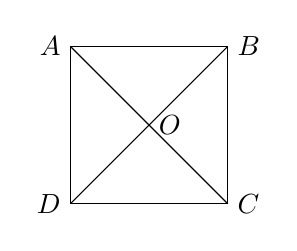
\begin{tikzpicture}
\draw (0,0) node[below,left] {$D$} -- (2,0) node[below,right] {$C$} -- (2,2) node[above,right] {$B$} -- (0,2) node[above,left] {$A$} -- cycle; 
\draw (0,0) -- (2,2);
\draw (0,2) -- (2,0);
\draw (1,1) node[right] {$O$};
\end{tikzpicture}\end{center}
\begin{enumerate}
 \item Quelle est la valeur de $p_0$ ?
 \item Déterminer une relation de récurrence entre $p_n$ et $p_{n+1}$.
 \item En déduire $p_n$ en fonction de $n$.
 \item Interpréter la limite de la suite $(p_n)_{n\in \N^*}$.
\end{enumerate}
\end{Exercice}


\begin{Exercice}{} Dans une zone d\'esertique, un animal erre entre trois points d'eau $A, B$ et $C.$
A l'instant $t=0,$ il se trouve au point $A.$

\noindent Quand il a \'epuis\'e l'eau du point o\`u il se trouve, il part avec \'equiprobabilit\'e rejoindre l'un des deux autres points d'eau.

\noindent L'eau du point qu'il vient de quitter se r\'eg\'en\`ere alors.


Soit $n\in\N.$ On note :

\begin{itemize}

\item[$\bullet$] $A_n$ l'\'ev\'enement \og l'animal est en $A$ apr\`es son $n$-i\`eme trajet \fg.


\item[$\bullet$] $B_n$ l'\'ev\'enement \og l'animal est en $B$ apr\`es son $n$-i\`eme trajet \fg.


\item[$\bullet$] $C_n$ l'\'ev\'enement \og l'animal est en $C$ apr\`es son $n$-i\`eme trajet \fg.

\end{itemize}

\noindent On pose aussi, $a_n=P(A_n), b_n=P(B_n)$ et $c_n=P(C_n).$



\begin{enumerate}

	\item 
	\begin{enumerate}
		\item Exprimer $a_{n+1}$ en fonction de $b_n$ et $c_n.$
		
		\item Exprimer de m\^eme $b_{n+1}$ et $c_{n+1}$ en fonction de $a_n, b_n$ et $c_n.$
		
	\end{enumerate}
	
	\item On consid\`ere $A=\left(\begin{array}{ccc}
	0 & 1/2 & 1/2\\
	1/2 & 0 & 1/2\\
	1/2 & 1/2 & 0\end{array}\right) \cdot$
	
	D\'eterminer une matrice $P$ inversible et une matrice $D$ diagonale telles que $D=P^{-1}AP.$
	
	
	\item Expliquer comment on pourrait obtenir explicitement $a_n$, $b_n$ et $c_n$ en fonction de $n.$
	
	
	
	
\end{enumerate}
\end{Exercice}



\begin{Exercice}{} On lance indéfiniment 3 dés équilibrés simultanément. Pour tout $n \geq 1$, on note $A_n$ l'évènement \og on obtient une triple 6 pour la première fois au $n$-ième tirage \fg . Déterminer $P(A_n)$ pour tout $n \geq 1$ et en déduire la probabilité d'obtenir au moins une fois un triple $6$.
\end{Exercice}



\begin{Exercice}{} On lance deux dés équilibrés jusqu'à ce que la somme des numéros obtenus soit un multiple de $5$. 
\begin{enumerate}
\item 
\begin{enumerate}
\item Soit $n \in \mathbb{N}^*$.  Donner la probabilité que l'épreuve s'arrête au $n$-ième lancer sur une somme égale à $5$ (on pourra noter $A_n$ cet évènement).
\item Donner la probabilité que l'épreuve s'arrête sur une somme égale à 5.
\end{enumerate}
\item Donner la probabilité que l'épreuve s'arrête par l'obtention d'un 10.
\item L'épreuve peut-elle ne jamais s'arrêter?
\end{enumerate}
\end{Exercice}


\begin{Exercice}{} On lance une infinité de fois une pièce équilibrée. On note pour tout $n \in \mathbb{N}^*$, $A_n$ l'évènement \og on obtient au moins une fois la séquence pile pile face au cours des $n$ premiers lancers \fg et $P_n$  l'évènement \og on obtient pile au $n$-ième lancer \fg .

\begin{enumerate}
\item Donner $P(A_1)$, $P(A_2)$ et $P(A_3)$.
\item Soit $n$ un entier supérieur ou égal à 4.
\begin{enumerate}
\item Montrer que $A_{n+1} = A_n  \cup (\overline{A_{n-2}} \cap P_{n-1} \cap P_n \cap \overline{P_{n+1}})$.
\item En déduire un lien entre $P(A_{n+1})$, $P(A_n)$ et $P(A_{n-2})$. 
\item Montrer que la suite $(P(A_n))_{n \geq 4}$ est croissante. Est-elle convergente ? Si oui, donner sa limite.
\item Montrer que la famille d'évènements $(A_n)_{n \geq 0}$ est croissante. En déduire $\dis P \bigg{(} \bigcup_{n=1}^{+  \infty} A_n \bigg{)}$. Qu'en déduit-on ?
\end{enumerate}
\end{enumerate}
\end{Exercice}


\begin{Exercice}{}
Soit $p \in ]0,1[$. On note $q=1-p$.\\
On effectue une infinité de lancers indépendants d'une pièce pour laquelle la probabilité d'obtenir Face est $p$.
\begin{enumerate}
\item Pour tout $n \in \mathbb{N}^*$, on note $A_n$ l'événement \og Au cours des $n$ premiers lancers, Face n'est jamais suivi de Pile\fg.
Montrer que :
$$P(A_n)=\begin{cases}
{\frac{p^{n+1}-q^{n+1}}{p-q}} & \text{si } p \neq \frac 1 2\\
{\frac{n+1}{2^n}} & \text{si } p=\frac 1 2
\end{cases}$$
\item Est-il possible que Face ne soit jamais suivi de Pile ?\\
Calculer la probabilité de l'événement $A$ : \og Face n'est jamais suivi de Pile \fg.
\end{enumerate}
\end{Exercice}



\begin{Exercice}{} Un enfant lance un galet pour faire des ricochets sur l'eau. On suppose que la probabilité que le galet ricoche pour la $n$-ième fois sachant qu'il a ricoché les $(n-1)$ coups d'avant, est égale à $\dis \frac{1}{n}\cdot$ On suppose que lors du premier coup, le galet ricoche nécessairement.
\begin{enumerate}
\item Soit $n \in \mathbb{N}^*$. Déterminer la probabilité $p_n$ que le galet coule après $n$ ricochets réussis.
\item Montrer que $\dis \sum_{n \geq 1} p_n$ converge, donner sa somme et interpréter.
\end{enumerate}
\end{Exercice}



\begin{Exercice}{} On effectue une succession infinie de lancers indépendants d'une pièce
donnant Pile avec la probabilité $p\in ]0,1[$ et Face avec la probabilité $%
q=1-p$.\newline
On s'intéresse dans cet exercice aux successions de lancers amenant un mê%
me côté.\newline
On dit que la première série est de longueur $n\geq 1$ si les $n$
premiers lancers ont amené le même côté de la pièce et le $(n+1)$-ième
l'autre côté.\newline
De même la deuxième série commence au lancer suivant la fin de la première sé%
rie et se termine (si elle se termine) au lancer précédant un changement de c%
ôté.\newline


\begin{enumerate}
\item Pour tout $n \in \mathbb{N}^*$, on note $A_n$ l'évènement \og La longueur de la première série est égale à $n$ \fg. Déterminer $P(A_n)$.
\item Montrer que :
\[\sum\limits_{n=1}^{+\infty }P(A_n)=1\]
Quelle est la probabilité que la première série ne se termine pas?

\item Pour $n \in \mathbb{N}^*$, on note $B_n$ l'évènement \og La longueur de la deuxième série est égale à $n$ \fg .

\begin{enumerate}
\item Déterminer pour $(n,k) \in (\mathbb{N}^*)^2$, $P(A_n \cap B_k)$.

\item En déduire que, pour $k\in \mathbb{N}^{* }$, $P(B_k)$.
\end{enumerate}
\end{enumerate}
\end{Exercice}


\medskip

\begin{center}
\textit{{ {\large Divers}}}
\end{center}

\medskip


\begin{Exercice}{\ding{80}}  Soit $(A_n)_{n \geq 0}$ une famille d'évènements mutuellement indépendants d'un même espace probabilisé.
\begin{enumerate}
\item On suppose que $\dis \sum_{n \geq 0} P(A_n)$ converge. Montrer que :
$$ \P \left( \bigcap_{n \geq 0} \overline{A_n} \right) \leq \exp \left(- \sum_{k=0}^{+ \infty} \P(A_k) \right)$$
\item On suppose que $\dis \sum_{n \geq 0} P(A_n)$ diverge. Montrer que :
$$ \P \left( \bigcap_{n \geq 0} \overline{A_n} \right) = 0$$
\end{enumerate}
\end{Exercice}



\begin{Exercice}{} Soit $(A_n)_{n \geq 0}$ une suite d'évènements d'un même espace probabilisé ayant tous probabilité 1. 
 
 \begin{enumerate}
 \item Montrer que $\P \left( \bigcup_{n \geq 0} \overline{A_n} \right) = 0$.
 \item Qu'en déduit-on pour $\P \left( \bigcap_{n \geq 0} A_n \right)$?
 \end{enumerate}
 \end{Exercice}
 

\end{document}